\chapter{Penggalian Data}
\label{chap:penggalian data}
Pada bab ini akan dijelaskan analisis masalah penelitian ini. Analisis meliputi Langkah-Langkah Query Yang Dilakukan Dengan Data Yang Lebih Besar. Query yang dilakukan sama dengan bab sebelumnya \ref{langkah_query} tetapi tidak menggunakan limit.

\section{Langkah-Langkah Query Yang Dilakukan Dengan Data Yang Lebih Besar}
Pada section ini akan dijelaskan tentang langkah-langkah query yang dilakukan dalam memperoleh data dan analisis yang dilakukan. Data yang diambil adalah semua data yang akan didapatkan dengan menggunakan \textit{query}. Data yang diambil merupakan dataset dari tabel technologies 2020$\_$08$\_$01:

\subsection{Mengumpulkan List Website}
Langkah pertama yang dilakukan yaitu mengumpulkan website. Website yang dicari tidak berdasarkan berdasarkan \textit{rank} karena tidak tersedia pada dataset tersebut. Berikut adalah \textit{query} yang digunakan untuk mengumpulkan list website.
\begin{lstlisting}
	SELECT url
	FROM `httparchive.technologies.2020_08_01_*`
	ORDER BY url asc
\end{lstlisting}

\subsection{Mencari Aplikasi Yang Digunakan Website}
Setiap website akan dicari aplikasi apa saja yang digunakan dalam pembangunan website tersebut dan versi dari aplikasi yang dipakainya. Berikut adalah query yang digunakan.
\begin{lstlisting}
	SELECT url, app, info
	FROM `httparchive.technologies.2020_08_01_*`
	ORDER BY url asc
\end{lstlisting}

\subsection{Mengelompokkan Berdasarkan Nama Semua Aplikasi Yang Dipakai}
Pengelompokan aplikasi dapat dilakukan dengan menggunakan query. Berikut adalah query yang digunakan.
\begin{lstlisting}
	SELECT tabelName.app, num.num_sites , versioned.versioned_count , unversioned.unversioned_count
	FROM 
	(SELECT DISTINCT app
	FROM `httparchive.technologies.2020_08_01_*` ) tabelName
	
	LEFT JOIN 
	
	(SELECT tabel1.app, count(app) AS versioned_count
	FROM `httparchive.technologies.2020_08_01_*` AS tabel1
	WHERE tabel1.app!="" AND tabel1.info != "" 
	GROUP BY tabel1.app) AS versioned
	
	ON(versioned.app = tabelName.app)
	
	LEFT JOIN
	
	(SELECT tabel2.app, count(app) AS unversioned_count
	FROM `httparchive.technologies.2020_08_01_*` AS tabel2
	WHERE tabel2.app!="" AND tabel2.info = "" 
	GROUP BY tabel2.app) AS unversioned
	
	ON (unversioned.app = tabelName.app)
	
	LEFT JOIN 
	
	(SELECT app, count(url) AS num_sites
	FROM `httparchive.technologies.2020_08_01_*`
	GROUP BY app) AS num
	
	ON (tabelName.app = num.app)
\end{lstlisting}

\subsection{Mencari Data Tentang Versi Aplikasi Yang Masih Didukung}
Sebelum menentukan suatau aplikasi usang atau tidak, kita harus mencari versi dari setiap aplikasi secara manual. Versi setiap aplikasi dapat dilihat di-\textit{official documentation} dari setiap aplikasi. Hasil pencarian dari aplikasi yang masih didukung dapat dilihat pada gambar \ref{lamp:A}. 

\subsection{Melakukan Perbandingan Antara Versi Aplikasi Yang Masih Dipakai Sekarang Dengan Versi Aplikasi Yang Masih Didukung}
Setelah mendapatkan data versi minimal dari setiap aplikasi, data tersebut akan dibandingkan dengan versi aplikasi yang dipakai \textit{url}. \textit{supported} adalah versi aplikasi dari yang dipakai url masih mendukung atau diatas atau sama dengan versi yang didukung didokumen. \textit{unsupported} adalah versi aplikasi dari yang dipakai url sudah tidak mendukung atau dibawah versi yang didukung didokumen. \textit{not\_versioned} adalah versi aplikasi dari url tidak ditampilkan. \textit{non\_conclusive} adalah versi aplikasi tidak dapat ditentukan. Data diambil berdasarkan banyak aplikasi yang dipakai oleh url tertentu. Data yang sudah dibandingkan juga digunakan untuk mencari jumlah website yang jumlah semua aplikasinya yang masih didukung. Terdapat 4.511 jumlah aplikasi yang digunakan website. Berikut adalah \textit{query} yang digunakan untuk mencari datanya:

\begin{lstlisting}
	SELECT url1.url, url1.jumlah1, url2.jumlah2
	FROM 
	(
	SELECT url, count(app) AS jumlah1
	FROM `skripsi2-327310.app_all.url_app_supported_unsupported`
	WHERE result = "SUPPORTED"
	GROUP BY url
	ORDER YB url ASC
	) AS url1
	
	JOIN 
	
	(
	SELECT url, count(app) AS jumlah2
	FROM `skripsi2-327310.app_all.url_app_supported_unsupported`
	GROUP BY url
	ORDER BY url ASC
	) AS url2
	
	ON url1.url = url2.url
	WHERE url1.jumlah1  = url2.jumlah2 
\end{lstlisting}
\textit{Project} skripsi2-327310 dengan nama dataset app\_all dan tabel url\_app\_supported\_unsupported adalah sebuah tabel pembantu. Project skripsi2-327310 ini dibuat berdasarkan data dari \textit{project} httparchive, dataset technologies, dan tabel 2020\_08\_01\_* yang kemudian dibuat tabel baru agar \textit{query} tidak dipanggil beberapa kali. \\
Pada \textit{query} diatas awalnya dibuat sebuah tabel yang bersifat sementara. Tabel diambil dari  \textit{project} skripsi2-327310 dengan nama dataset app\_all dan tabel url\_app\_supported\_unsupported. Pada tabel ini akan dicari url dan data dengan informasi versi dari aplikasi yang masih didukung url tersebut, tabel diberi nama url1. Kemudian tabel akan digabungkan dengan tabel lain yang bersifat sementara. Pada tabel ini dicari semua url dan jumlah aplikasi yang dipakai oleh url tersebut, tabel diberi nama url2. Hasil akhir dari \textit{query} ini berupa url yang dan jumlah dari tabel url1 dan tabel url2.


\section{Hasil Sample Data}
Data yang ditampilkan adalah data beberapa aplikasi yang sudah dipisahkan berdasarkan aplikasi dan nomor versi dari aplikasi yang dipakai serta jumlahnya dalam bentuk \textit{chart}.

\subsection{Apache dan Nginx}
Apache dan Nginx merupakan dua web servers yang paling banyak digunakan. Pada dua web servers ini, aplikasi Apache memiliki lebih banyak jumlah yang supported daripada aplikasi Nginx. Pada aplikasi Nginx terdapat 5.440.268 aplikasi yang \textit{unversioned}. Versi pada aplikasi Nginx yang paling banyak digunakan adalah versi 1.16.1 dengan jumlah 267.102. Pada aplikasi Apache terdapat 2.949.180 aplikasi yang \textit{unversioned}. Versi pada aplikasi Apache yang paling banyak digunakan adalah versi 2 dengan jumlah 154.533. Berikut ini adalah chart yang dapat dilihat pada gambar \ref{fig:data_sample_nginx} dan \ref{fig:data_sample_apache}:
\begin{figure}[H]
	\centering  
	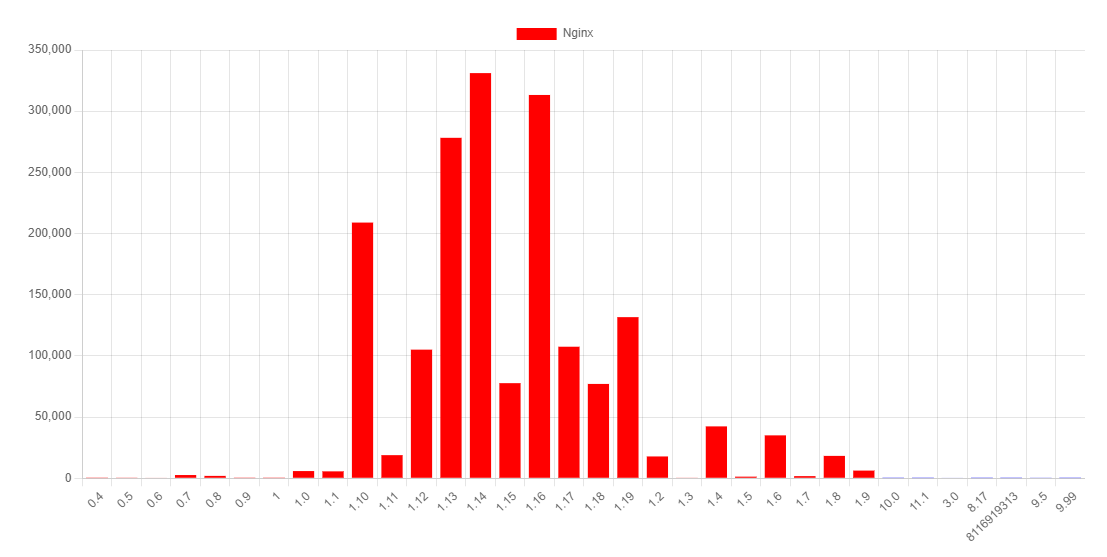
\includegraphics[scale=0.4]{Gambar/data_sample_nginx.png}  
	\caption{Aplikasi Nginx} 
	\label{fig:data_sample_nginx} 
\end{figure}

\begin{figure}[H]
	\centering  
	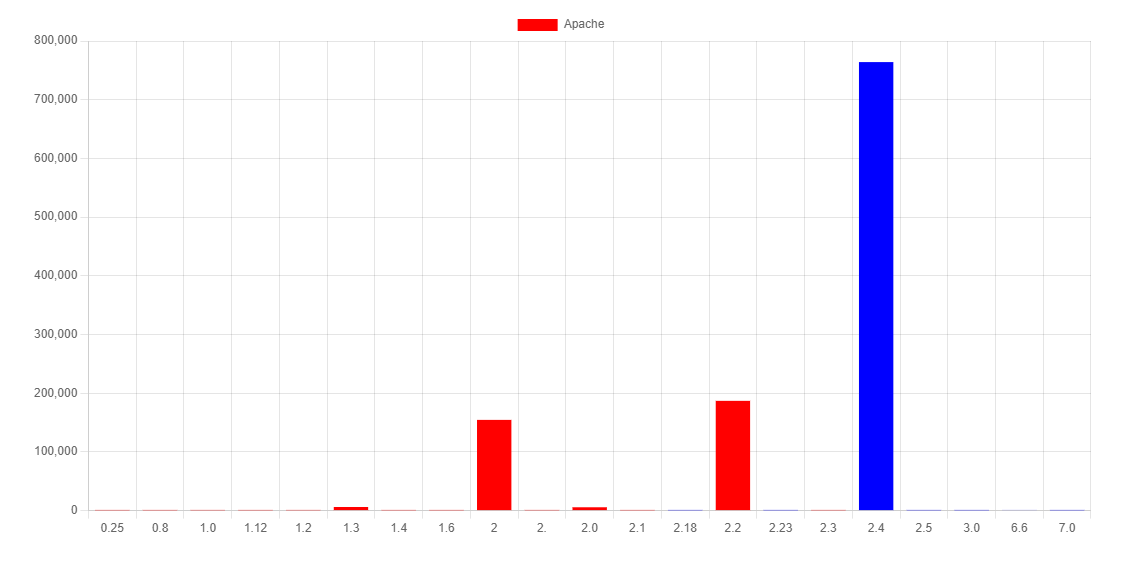
\includegraphics[scale=0.4]{Gambar/apache.png}  
	\caption{Aplikasi Apache} 
	\label{fig:data_sample_apache} 
\end{figure}

Berdasarkan penelitian dengan aplikasi yang sama, didapatkan hasil dalam bentuk chart. Chart yang dibandingkan dapat dilihat pada gambar \ref{fig:data_sample_apache_p} dan gambar \ref{fig:data_sample_nginx_p}.
\begin{figure}[H]
	\centering  
	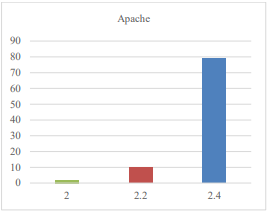
\includegraphics[scale=0.7]{Gambar/chart_pascal_apache.PNG}  
	\caption{Aplikasi Apache dari \cite{pascal}} 
	\label{fig:data_sample_apache_p} 
\end{figure}
\begin{figure}[H]
	\centering  
	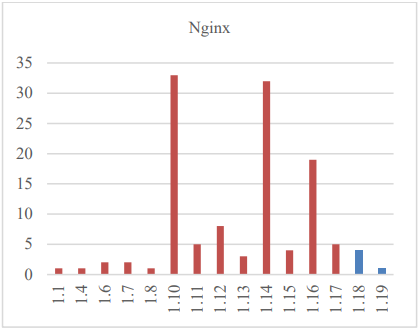
\includegraphics[scale=0.7]{Gambar/chart_pascal_nginx.PNG}  
	\caption{Aplikasi Apache dari \cite{pascal}} 
	\label{fig:data_sample_nginx_p} 
\end{figure}

\subsection{PHP dan Python}
PHP merupakan bahasa pemograman yang digunakan dalam pembuatan website. PHP manjadi bahasa pemograman yang paling banyak digunakan. Pada aplikasi PHP terdapat 3.455.170 aplikasi yang \textit{unversioned}. Versi pada aplikasi PHP yang paling banyak digunakan adalah versi 5.6.40 dengan jumlah 358.750.
Python meruapakan bahasa pemograman tingkat tinggi dan berorientasi objek. Python adalah bahasa pemograman tingkat tinggi karena perintah atau kode program yang digunakan sudah mirip dengan bahasa manusia. Pada aplikasi Python terdapat 360.531 aplikasi yang \textit{unversioned}. Versi pada aplikasi Python yang paling banyak digunakan adalah versi 2.7.5 dengan jumlah 7.481. Berikut ini adalah chart yang dapat dilihat pada gambar \ref{fig:data_sample_php} dan \ref{fig:data_sample_python}:
\begin{figure}[H]
	\centering  
	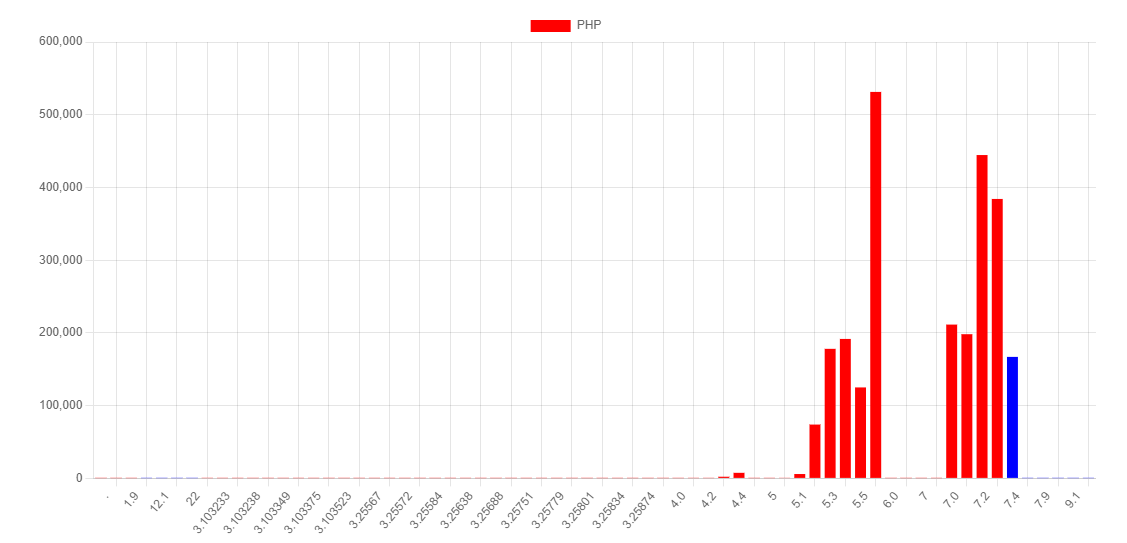
\includegraphics[scale=0.4]{Gambar/data_sample_php.png}  
	\caption{Aplikasi PHP} 
	\label{fig:data_sample_php} 
\end{figure}

\begin{figure}[H]
	\centering  
	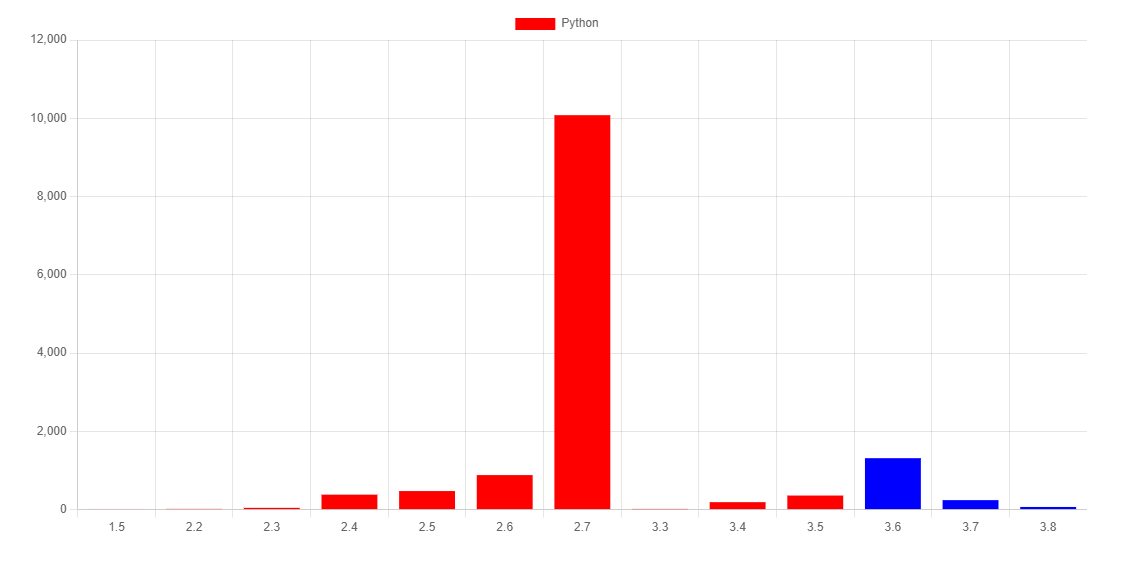
\includegraphics[scale=0.4]{Gambar/data_sample_python.png}  
	\caption{Aplikasi Python} 
	\label{fig:data_sample_python} 
\end{figure}

Berdasarkan penelitian dengan aplikasi yang sama, didapatkan hasil dalam bentuk chart. Chart yang dibandingkan dapat dilihat pada gambar \ref{fig:data_sample_php_p}.

\begin{figure}[H]
	\centering  
	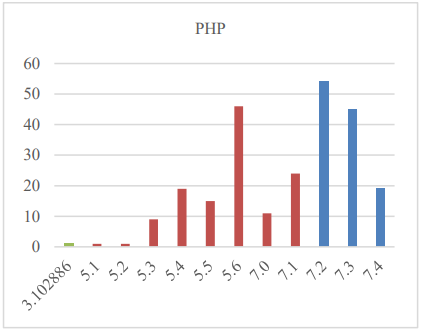
\includegraphics[scale=0.7]{Gambar/chart_pascal_php.PNG}  
	\caption{Aplikasi PHP dari \cite{pascal}} 
	\label{fig:data_sample_php_p} 
\end{figure}

\subsection{jQuery dan jQuery Migrate}
jQuery dan jQuery Migrate merupakan \textit{javascipt libraries} yang paling banyak digunakan. jQuery berfungsi untuk membantu mengatur interaksi antara javascript dan html pada sisi \textit{client}. Pada aplikasi jQuery terdapat 24.029 aplikasi yang \textit{unversioned}. Versi pada aplikasi jQuery yang paling banyak digunakan adalah versi 1.12.4 dengan jumlah 3.603.522. jQuery Migrate berfungsi untuk membantu memulihkan API yang telah dihapus dan menunjukkan peringatan pada \textit{browser concole}. Pada aplikasi jQuery Migrate terdapat 268.962 aplikasi yang \textit{unversioned}. Versi pada aplikasi jQuery yang paling banyak digunakan adalah versi 1.4.1 dengan jumlah 2.935.408. Hasil chart dapat dilihat pada gambar \ref{fig:data_sample_jQuery} dan  \ref{fig:data_sample_jQuery_migrate}
\begin{figure}[H]
	\centering  
	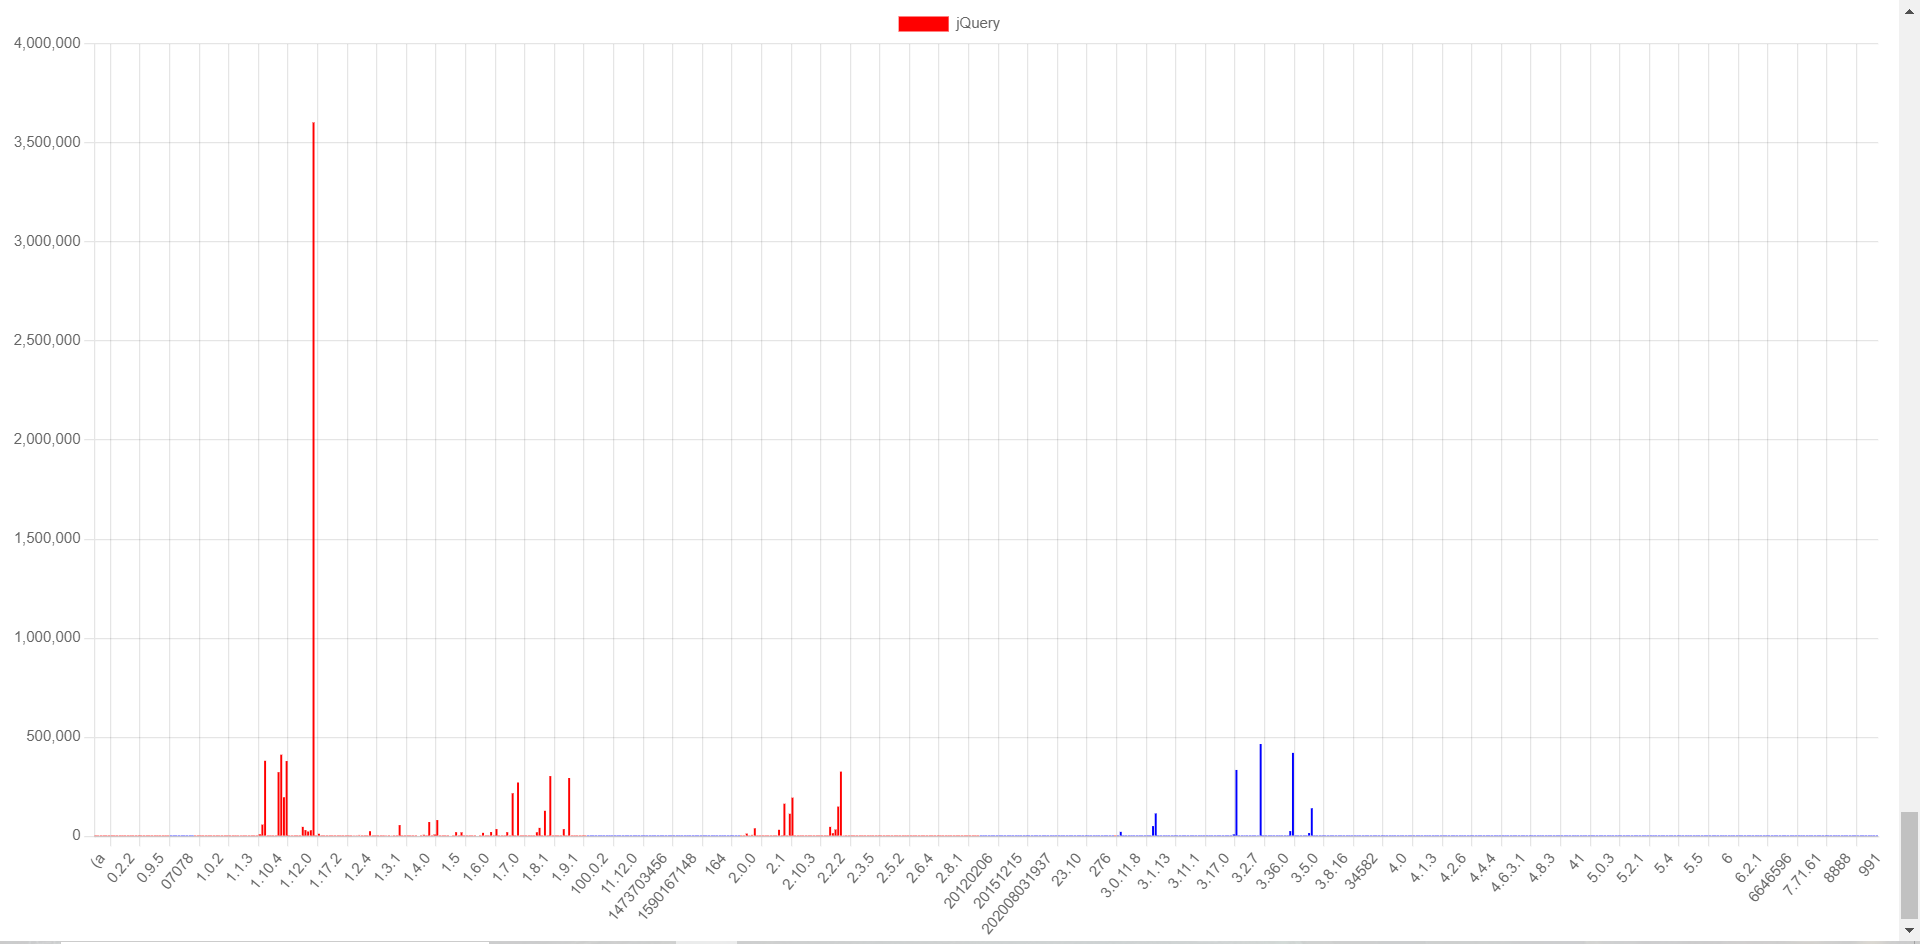
\includegraphics[scale=0.4]{Gambar/data_sample_jQuery.png}  
	\caption{Aplikasi jQuery} 
	\label{fig:data_sample_jQuery} 
\end{figure}

\begin{figure}[H]
	\centering  
	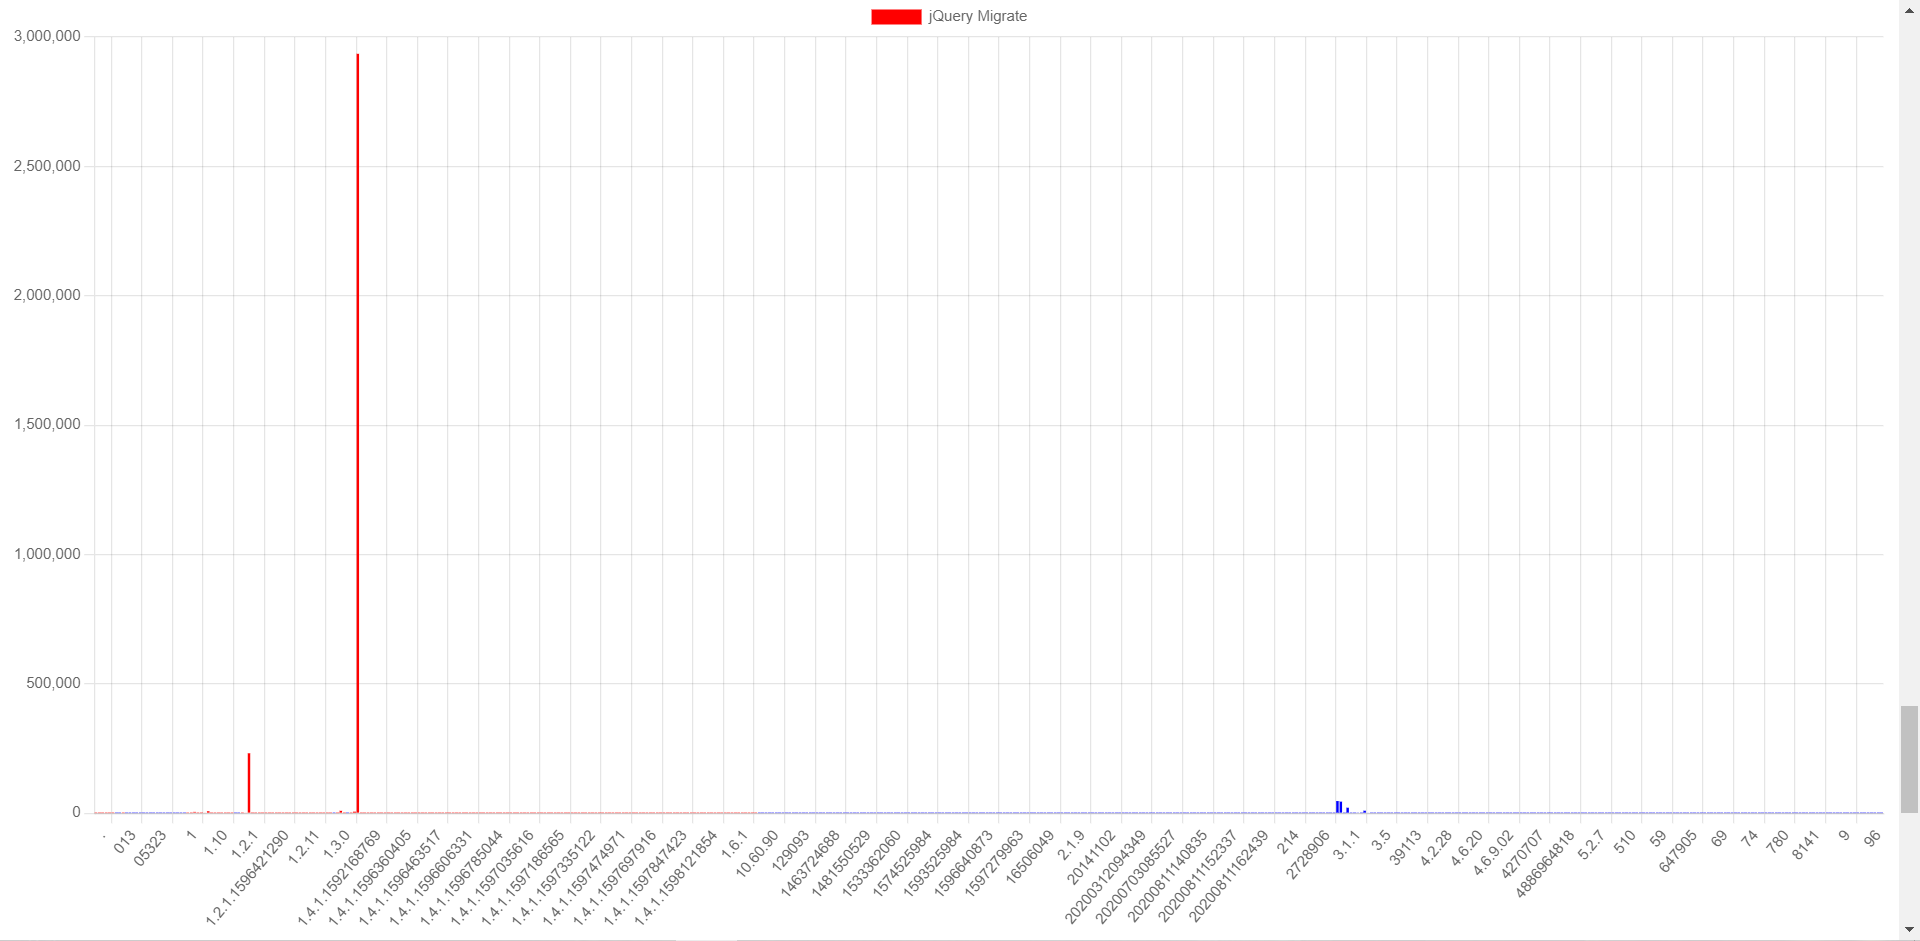
\includegraphics[scale=0.7]{Gambar/data_sample_jQuery_migrate.png}  
	\caption{Aplikasi jQuery Migrate} 
	\label{fig:data_sample_jQuery_migrate} 
\end{figure}

Berdasarkan penelitian dengan aplikasi yang sama, didapatkan hasil dalam bentuk chart. Chart yang dibandingkan dapat dilihat pada gambar \ref{fig:data_sample_jQuery_p}.

\begin{figure}[H]
	\centering  
	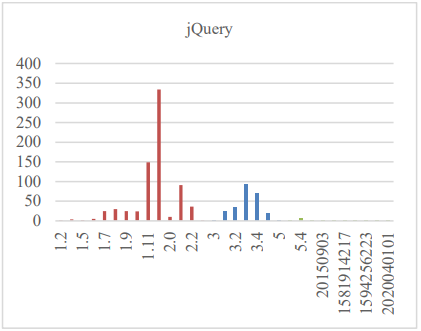
\includegraphics[scale=0.7]{Gambar/chart_pascal_jQuery.PNG}  
	\caption{Aplikasi jQuery dari \cite{pascal}} 
	\label{fig:data_sample_jQuery_p} 
\end{figure}